%%%% This Beamer example was created by LianTze Lim, April 2017.

%%%% This is a VERY simple and minimalistic beamer theme,
%%%% even reminiscent of marker pens on transparencies!
%%%% It mimics the look of the "seminar" package, which
%%%% can only be used with plain TeX.
%%%% There are also some comments and example to show how
%%%% to customise various elements, e.g. the font and colours.

\documentclass[12pt]{beamer}
%% If you'd like the default font size to be even larger, use 14pt or 17pt; these are supported by Beamer.

\usepackage[english]{babel}
\usepackage[utf8]{inputenc}
\usepackage[T1]{fontenc}
\usepackage{lmodern}
\usepackage{tikz}
\usepackage{graphicx}
\graphicspath{ {./images/} }
\usepackage{amsmath}% http://ctan.org/pkg/amsmath

%%%%%%%%%%%%%%%%%%%%%%%%%%%%%%%%%%%%%%%%%
% These lines should usually go into a .sty file,
% but I'll leave them here so that it's easier to
% see how to customise a Beamer theme.
% Remember, the Beamer manual is your friend!!
% http://texdoc.net/pkg/beamer
%
%% So if your re-definitions have a @ somewhere, you
%% _MUST_ put a \makeatletter before these lines and then
%% \makeatother after them. This trick can only be done
%% in the preamble! BUT if you're doing these re-definitions
%% in a .sty file (so that you \usepackage it later), you
%% don't need the \makeatletter and \makeatother.
\makeatletter

%% Set the left and right margins
\setbeamersize{text margin left=1em,text margin right=1em}

%% FONTS
\setbeamerfont{title}{series=\bfseries,size=\LARGE}
\setbeamerfont{subtitle}{series=\bfseries,size=\Large}
\setbeamerfont{frametitle}{series=\bfseries,size=\small}
\setbeamerfont{block title}{series=\bfseries,size=\normalsize}
\setbeamerfont{footline}{size=\normalsize}

%% COLOURS
%% If you'd like everything to have the same colour
\usebeamercolor{structure}
\setbeamercolor{normal text}{fg=structure.fg}

%% Add a line after the frametitle
\addtobeamertemplate{frametitle}{}{\vspace*{-1ex}\rule{\textwidth}{1pt}}

%% Use circular discs as itemized list markers;
%% there's an existing option in Beamer for it so I'll use it
\setbeamertemplate{itemize items}[circle]

%% Remove default navigation symbols (We'll add the ones we need in the footline
\setbeamertemplate{navigation symbols}{}

\makeatother
%%%% END STYLE CUSTOMISATION %%%%%%%%%%%%



\title{Komplexe Fourierreihe}
\subtitle{Von der Akustik zum komplexen Zeichnen}
\author{GFS – Maximilian}

\begin{document}

\begin{frame}
  \titlepage
\end{frame}

\begin{frame}{Hinführung}
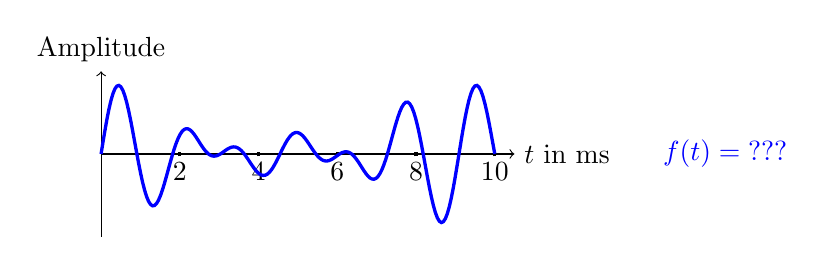
\begin{tikzpicture}[domain=0:10, samples=200, xscale=0.5, yscale=0.3]
  \draw[->] (0,0) -- (10.5,0) node[right] {$t$ in ms};
  \draw[->] (0,-3.5) -- (0,3.5) node[above] {Amplitude};
  \foreach \t in {2, 4, ..., 10}  
    \draw[very thick] (\t,-.1) -- (\t,.1) node[below] {\t};

  \draw[color=blue, very thick] plot (\x,{sin(360*0.44*\x) + sin(360*0.55*\x) + sin(360*0.66*\x)})  node[right=2cm] {$f(t) = \text{???}$};
\end{tikzpicture}

\pause

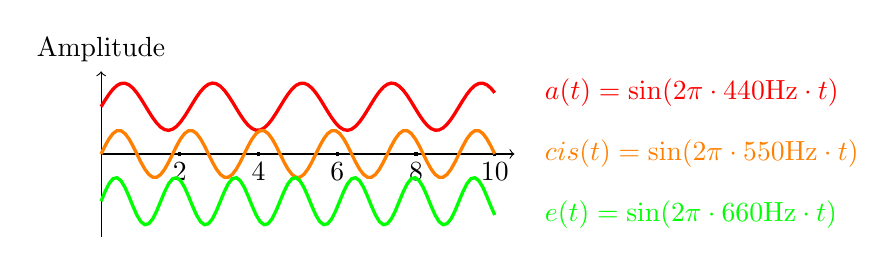
\begin{tikzpicture}[domain=0:10, samples=100, xscale=0.5, yscale=0.3]
  \draw[->] (0,0) -- (10.5,0);
  \draw[->] (0,-3.5) -- (0,3.5) node[above] {Amplitude};
  \foreach \t in {2, 4, ..., 10}  
    \draw[very thick] (\t,-.1) -- (\t,.1) node[below] {\t};
  
  \draw[color=red, very thick] plot (\x,{sin(360*0.44*\x)+2}) node[right=.5cm] {$a(t) = \sin (2\pi \cdot 440 \text{Hz} \cdot t)$};

  \pause
  
  \draw[color=orange, very thick] plot (\x,{sin(360*0.55*\x)}) node[right=.5cm] {$cis(t) = \sin (2\pi \cdot 550 \text{Hz} \cdot t)$};  

  \pause
  
  \draw[color=green, very thick] plot (\x,{sin(360*0.66*\x)-2}) node[right=.5cm] {$e(t) = \sin (2\pi \cdot 660 \text{Hz} \cdot t)$};
\end{tikzpicture}

$$f(t) = a(t) + cis(t) + e(t)$$
\end{frame}

\begin{frame}{Einleitung}
\begin{minipage}{0.79\linewidth}
	\begin{block}{Idee}
		Jede \textit{periodische} Funktion kann durch die \textit{Überlagerung von Sinus- und Kosinusfunktionen} dargestellt werden, deren \textit{Frequenzen Vielfache der Grundfrequenz} sind.
	\end{block}
\end{minipage}
\begin{minipage}{0.19\linewidth}
	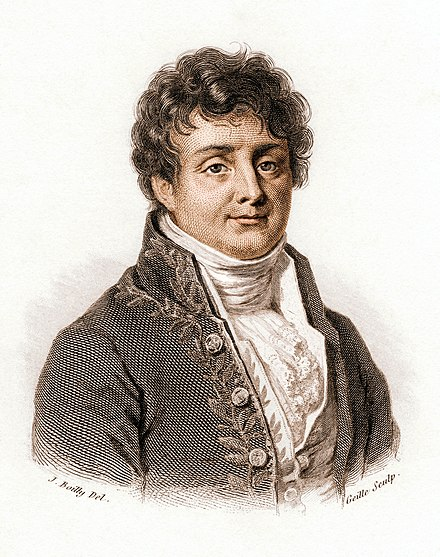
\includegraphics[width=\linewidth]{fourier.jpg}
\end{minipage}

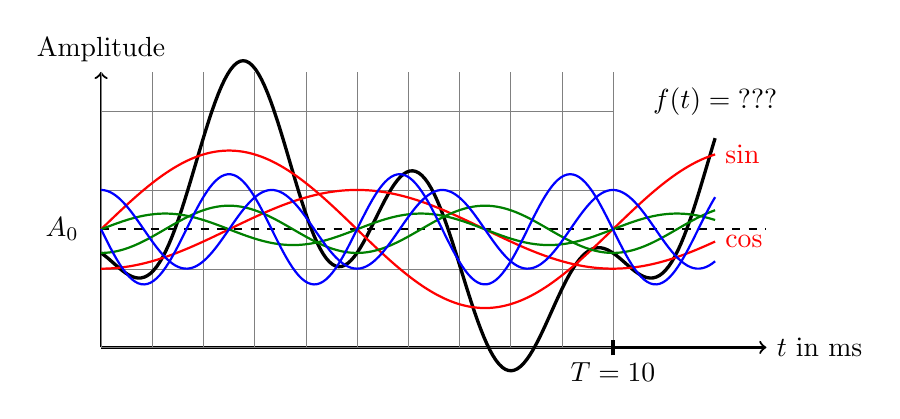
\begin{tikzpicture}[domain=0:12, samples=200, xscale=0.65, yscale=1]
  \draw[thick, ->] (0,0) -- (13,0) node[right] {$t$ in ms};
  \draw[thick, ->] (0,0) -- (0,3.5) node[above] {Amplitude};
  \draw[ultra thin, gray] (0,0) grid (10, 3.5);
  \draw[ultra thick] (10,-.1) -- (10,.1) node[below=1ex] {$T=10$};

  \draw[color=black, very thick] plot (\x,{1.5+sin(36*\x)-0.5*cos(36*\x)+0.2*sin(2*36*\x)-0.3*cos(2*36*\x)-0.7*sin(3*36*\x)+0.5*cos(3*36*\x)})  node[above=1ex] {$f(t) = \text{???}$};

  \pause

  \draw[thick, black, dashed] (0, 1.5) node[left=1ex] {$A_0$} -- ++(13,0);

  \pause
  
  \draw[color=red, thick] plot (\x,{1.5+sin(36*\x)}) node[right] {$\sin$};
  \draw[color=red, thick] plot (\x,{1.5-0.5*cos(36*\x)}) node[right] {$\cos$};

  \pause

  \draw[color=green!50!black, thick] plot (\x,{1.5+0.2*sin(2*36*\x)});
  \draw[color=green!50!black, thick] plot (\x,{1.5-0.3*cos(2*36*\x)});

  \pause

  \draw[color=blue, thick] plot (\x,{1.5-0.7*sin(3*36*\x)});
  \draw[color=blue, thick] plot (\x,{1.5+0.5*cos(3*36*\x)});
\end{tikzpicture}
\end{frame}

\begin{frame}{Reelle Fourierreihe}
	\vspace*{-1cm}
	\begin{align*}    
		s_N(t) &= A_0 \\
		&+ A_1 \cos(2\pi \frac{\mathbf{1}}{T} \cdot t) + B_1 \sin(2\pi \frac{\mathbf{1}}{T} \cdot t) \quad \text{Grundfrequenz} \\[1ex]
		&+ A_2 \cos(2\pi \frac{\mathbf{2}}{T} \cdot t) + B_2 \sin(2\pi \frac{\mathbf{2}}{T} \cdot t) \quad \text{2x Grundfrequenz} \\[1ex]
		&\;\vdots \quad\quad\quad \vdots \quad N \text{ mal...} \\
		&= A_0 + \sum_{n=1}^N \left(A_n \cos(2\pi \frac{n}{T} \cdot t) + B_n \sin(2\pi \frac{n}{T} \cdot t)\right)
	\end{align*}
	
	\pause
	\begin{align*}
		\lim_{N \rightarrow \infty} s_N(t) = \underbrace{A_0 + \sum_{n=1}^\infty \left(A_n \cos(2\pi \frac{n}{T} \cdot t) + B_n \sin(2\pi \frac{n}{T} \cdot t)\right)}_{\text{Reelle Fourierreihe}} = f(t).
	\end{align*}
\end{frame}

\begin{frame}{Simulation}
	\begin{minipage}{0.49\linewidth}
		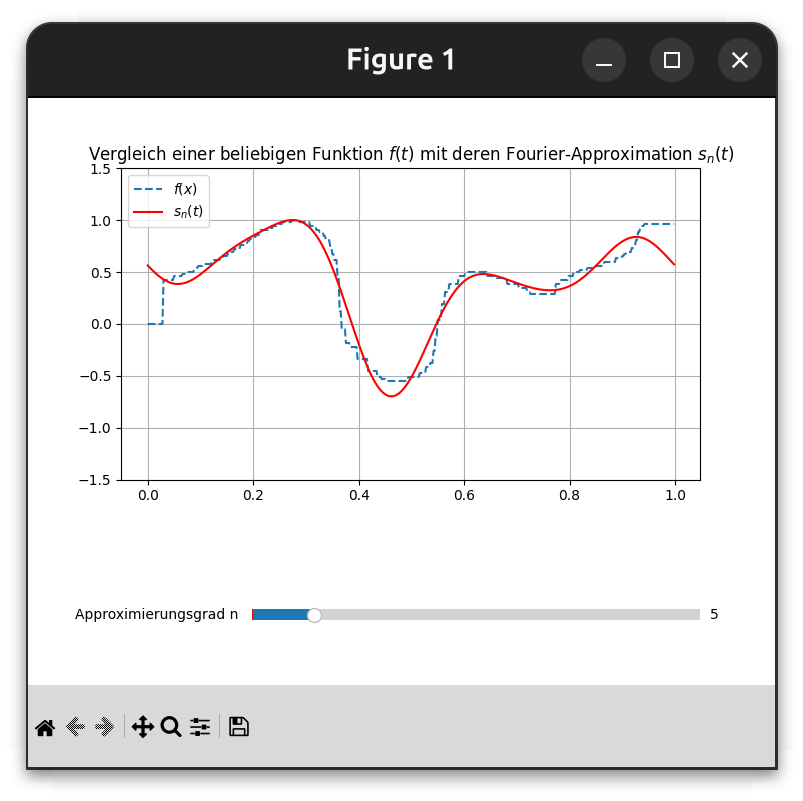
\includegraphics[width=\linewidth]{simscreenshot.png}
	\end{minipage}
	\begin{minipage}{0.39\linewidth}
		\begin{block}{Koeffizienten?}
			\vspace*{-1ex}
			\begin{align*}
				A_0 &= \frac{1}{T} \int_{0}^T f(t) \, dt \\[2ex]
				A_n &= \frac{2}{T} \int_{0}^T f(t) \cdot \cos(2\pi \frac{n}{T} \cdot t) \, dt \\[2ex]
				B_n &= \frac{2}{T} \int_{0}^T f(t) \cdot sin(2\pi \frac{n}{T} \cdot t) \, dt
			\end{align*}
			Die Integrale wurden numerisch bestimmt.
		\end{block}
	\end{minipage}
\end{frame}

\begin{frame}{Wiederholung der komplexen Zahlen}
    \begin{center}
        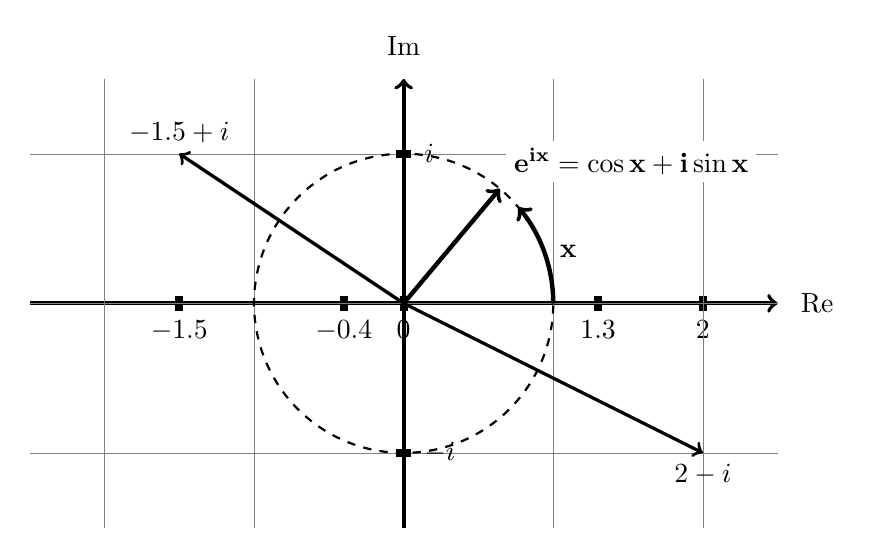
\begin{tikzpicture}[scale=1.9]
            \draw[line width=.5mm, ->] (-2.5,0) -- (2.5, 0) node[right=1ex] {Re};
            
            \pause
            
            \foreach \x in {-1.5,-0.4, 0, 1.3, 2} \draw[line width=1mm] (\x, -0.05) -- ++(0,0.1) node[below=1ex] {$\x$};

            \pause

            \draw[ultra thin, gray] (-2.5,-1.5) grid (2.5,1.5);
            \draw[line width=.5mm, ->] (0,-1.5) -- (0, 1.5) node[above=1ex] {Im};
            
            \draw[line width=1mm] (-0.05, -1) -- ++(0.1, 0) node[right] {$-i$};
            \draw[line width=1mm] (-0.05, 1) -- ++(0.1, 0) node[right] {$i$};

            \pause

            \draw[very thick, ->] (0,0) -- (-1.5, 1) node[above] {$-1.5+i$};
            \draw[very thick, ->] (0,0) -- (2, -1) node[below] {$2-i$};

            \pause

            \draw[dashed, thick] (0,0) circle (1);
            \draw[ultra thick, ->] (0,0) -- (50:1);
            \draw[ultra thick, ->] (1,0) arc (0:40:1);
            \node at (1.1, 0.35) {$\mathbf{x}$};

            \pause
            
            \node[fill=white, inner sep=1mm, above right=.5ex] at (50:1) {$\mathbf{e^{ix} = \cos x + i \sin x}$};
        \end{tikzpicture}
    \end{center}
\end{frame}

\begin{frame}{Komplexe Zeiger}
	\begin{center}
		\vspace*{-1ex}
		Anfangskonfiguration $C_n \in \mathbb{C}$ und Freuqenz $f_n \in \mathbb{R}, [f] = 1 \text{Hz}$
		
		\vspace*{3ex}
		
		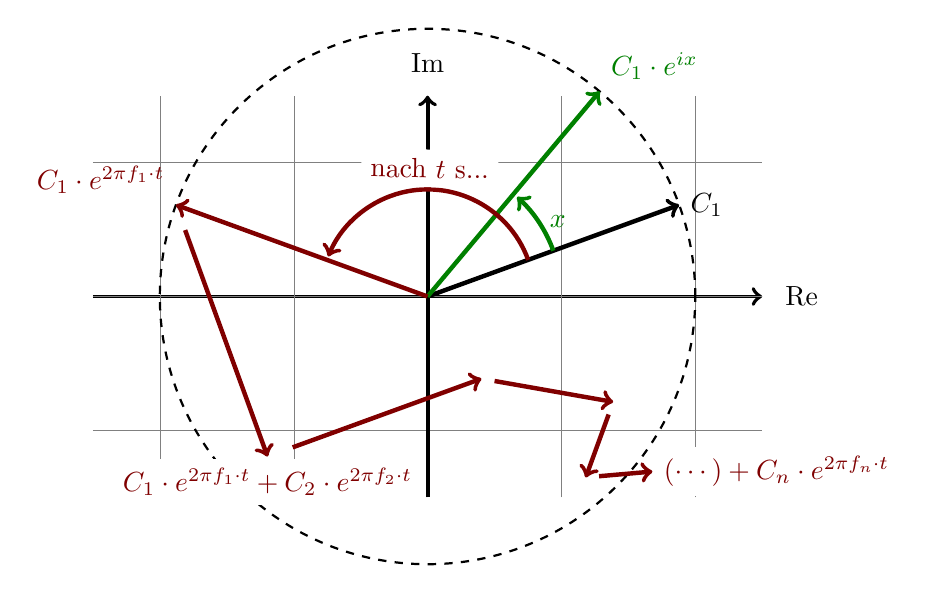
\begin{tikzpicture}[scale=1.7]
			\draw[line width=.5mm, ->] (-2.5,0) -- (2.5, 0) node[right=1ex] {Re};
			\draw[ultra thin, gray] (-2.5,-1.5) grid (2.5,1.5);
			\draw[line width=.5mm, ->] (0,-1.5) -- (0, 1.5) node[above=1ex] {Im};
			
			\pause
			
			\draw[dashed, thick] (0,0) circle (2);
			\draw[ultra thick, ->] (0,0) -- (20:2) node[right] {$C_1$};
			
			\pause
			
			\draw[ultra thick, green!50!black, ->] (20:1) arc (20:48:1) node[midway, right] {$x$};
			\draw[ultra thick, green!50!black, ->] (0,0) -- (50:2) node[above right] {$C_1 \cdot e^{i x}$};
			
			\pause
			
			\draw[ultra thick, red!50!black, ->] (20:.8) arc (20:158:.8) node[fill=white, midway, above, sloped] {nach $t$ s...};
			\draw[ultra thick, red!50!black, ->] (0,0) -- (160:2) node[above left] {$C_1 \cdot e^{2\pi f_1 \cdot t}$};
			
			\pause
			
			\draw[ultra thick, red!50!black, ->] (160:2) ++(-70:0.2) -- ++(-70:1.8) node[below, fill=white] {$C_1 \cdot e^{2\pi f_1 \cdot t} + C_2 \cdot e^{2\pi f_2 \cdot t}$};
			
			\pause
			
			\draw[ultra thick, red!50!black, ->] (160:2) ++(-70:2) ++(20:0.2) -- ++(20:1.5);
			\draw[ultra thick, red!50!black, ->] (160:2) ++(-70:2) ++(20:1.7) ++(-10:0.1) -- ++(-10:0.9);
			\draw[ultra thick, red!50!black, ->] (160:2) ++(-70:2) ++(20:1.7) ++(-10:1) ++(-110:0.1) -- ++(-110:0.5);
			\draw[ultra thick, red!50!black, ->] (160:2) ++(-70:2) ++(20:1.7) ++(-10:1) ++(-110:0.6) ++(5:0.1) -- ++(5:0.4) node[right, fill=white] {$(\cdots) + C_n \cdot e^{2\pi f_n \cdot t}$};
		\end{tikzpicture}
	\end{center}
\end{frame}

\end{document}
